\documentclass[a4paper,10pt]{article}
\usepackage[utf8]{inputenc}
\usepackage[spanish]{babel}
%links en el indice
\usepackage[bookmarks = true, colorlinks=true, linkcolor = black, citecolor = black, menucolor = black, urlcolor = black]{hyperref} 
\usepackage{graphicx}



%opening
\title{Triage, Sistema de gestión para sala de Guardia hospitalaria}
\author{Néstor Muñoz\\ Marcia Tejeda\\ \\ Director: Nicolás Páez \\  Co-Director: Pablo E. Martínez López}



\begin{document}



\maketitle
\newpage 
\begin{abstract}
El presente Trabajo de Inserción Profesional (TIP) se desarrolló en el contexto del desarrollo de un sistema para resolver necesidades de la guardia del Hospital Oñativia en Rafael Calzada.\\ 
El problema presentado en este TIP es automatizar la recepción en la guardia del Hospital utilizando el método de emergencias conocido como Triage.\\ 
La solución propuesta es el desarrollo de una aplicación web que sea accesible desde todos los puntos de atención de las guardias y que permita evaluar los casos que se presentan de manera eficiente y con los mismos parámetros.

\end{abstract}


\newpage 
\tableofcontents

\newpage

\newpage 
\section{Introducción}
\subsection{Contexto general}
Actualmente la guardia del H.Z.G.A ''Dr. Arturo Oñativia'' de la localidad de Rafael Calzada, a cargo del Doctor Luis Reggiani, utiliza el método Triage \cite{Derlet} \cite{Manual} para la clasificación de pacientes según los síntomas que presenten. Hasta el momento todo el proceso se hace en forma manual, lo que implica algunos contratiempos:
\begin{itemize}
\item Depender de una persona (o varias) con todo el conocimiento.
\item Emplear demasiado tiempo para guardar datos y recolectarlos.
\item Obtener diferentes resultados (algunas veces incorrectos), pues diferentes personas usan a veces criterios diferentes para la toma de decisiones.
\end{itemize}
Según Luis Reggiani informatizar el proceso de Triage implicaría una mejora notable en el desempeño de la guardia. Se lograría una estandarización en la clasificación de síntomas, se agilizaría el ingreso y la obtención de datos de pacientes, se mejoraría la atención en general y se distinguirían de una manera más eficaz aquellos pacientes que necesiten una atención inmediata.
\subsection{Sobre el TRIAGE}
Triage es un método de la medicina de emergencias y desastres para la selección y clasificación de los pacientes basándose en las prioridades de atención, privilegiando la posibilidad de supervivencia, de acuerdo a las necesidades terapéuticas y los recursos disponibles. Trata de evitar que se retrase la atención del paciente que empeoraría su pronóstico por la demora en su atención. Un nivel que implique que el paciente puede ser demorado no quiere decir que el diagnóstico final no pueda ser una enfermedad grave, ya que un cáncer, por ejemplo, puede tener funciones vitales estables que no lleve a ser visto con premura. El triage prioriza el compromiso vital inmediato y las posibles complicaciones.
\subsection{Propuesta de solución}
Proponemos desarrollar y poner en funcionamiento un sistema informático que dé soporte al proceso de Triage en la guardia del H.Z.G.A ''Dr. Arturo Oñativia'' de la localidad de Rafael Calzada.\\
Dado que el sistema podría incluir muchísimas funcionalidades y al mismo tiempo existe una especificación detallada de los requerimientos, planteamos el proyecto con alcance variable con el compromiso de entrega de un software que resuelva la parte central del proceso de Triage. La idea es que el sistema desarrollado en el contexto de este trabajo sea puesto en marcha y utilizado por la institución promotora.
\subsection{Objetivo General}
Concretamente el sistema debe cubrir las siguientes funcionalidades mínimas:
\begin{itemize}
\item Recepción de pacientes mediante búsqueda de aquellos que ya fueron atendidos en el hospital e ingreso de los que se atienden por primera vez.
\item Toma de impresión visual inicial del paciente.
\item Toma de los signos vitales que presenta el paciente: presión arterial (sístole y diástole), frecuencia cardíaca, saturación de O2, frecuencia respiratoria, temperatura y glucosa.
\item Ingreso de los síntomas que presenta el paciente.
\item División de los síntomas por categorías (discriminantes) y asociación de prioridades a los mismos.
\item Lógica variada para los síntomas, según se trate de un paciente adulto o pediátrico, tanto para los valores de los signos vitales como para las prioridades de los síntomas.
\item Emisión de alerta al momento de detectarse un síntoma de prioridad uno, para que se ingrese al paciente de inmediato al shock room.
\item Posibilidad de extraer reportes de cantidad de consultas realizadas según prioridad y promedio de tiempo de espera de atención según prioridad.
\item Puesta en funcionamiento en cada sala de recepción de pacientes de guardia.
\end{itemize}
\subsection{Resultado Final}
Desarrollamos una aplicación web que cubre todas las funcionalidades mínimas detalladas anteriormente y además realiza las siguientes:
\begin{itemize}
\item Generación de reportes por paciente a modo de historial de atenciones en guardia con detalle de fecha, síntomas presentados, signos vitales, prioridad asignada y tipo de atención recibida.
\item Diferenciación entre usuarios administradores del sistema y usuarios comunes.
\item Posibilidad de detallar el tipo de atención recibida por el paciente luego de pasar por el proceso de Triage
\item Alta, baja y modificación de pacientes, síntomas, discriminantes de síntomas y usuarios del sistema.
\end{itemize}
\subsection{Síntesis de trabajo}
TODO

\newpage 
\section{Planteo}

El presente trabajo comenzó con el relevamiento de información mediante reuniones con el Dr.\ Reggiani, con quien hubo contacto constante durante todo el desarrollo. Las primeras reuniones fueron para describir el problema y las necesidades reales. Luego, durante la etapa de desarrollo, cada pantalla y funcionalidad fue validada por el usuario, con el propósito de llegar a un producto que fuera útil y consistente. A medida que avanzamos con el producto, se fue negociando el alcance agregando o quitando funcionalidades dependiendo del tiempo disponible y consultando con el Dr.\ la prioridad para cada tarea.

En esta sección iremos presentando los resultados de estos encuentros.


\subsection{Dinámica de trabajo en el hospital}
La guardia del H.Z.G.A ``Dr.\ Arturo Oñativia'' opera recibiendo a los pacientes en dos sectores: Pediatría y Adultos. Cada sector tiene definidos sus parámetros de evaluación de pacientes, pudiendo un síntoma tener una prioridad para los adultos y otra para los pacientes pediátricos. Hay una división entre los pacientes pediátricos también dependiendo de la edad, diferenciando bebés de meses y niños más grandes.

Al llegar a la guardia los pacientes son recibidos por el enfermero de guardia, quién utilizando el sistema desarrollado toma una impresión visual del paciente. Luego se pasa a la sala de toma de signos vitales donde otro enfermero controla la presión, glucosa en sangre, entre otros, y graba en el sistema los síntomas que presenta el paciente. En caso de encontrar algún síntoma de prioridad UNO (peligro de muerte o daño permanente) en alguna de las tres instancias mencionadas antes (Impresión Visual, Signos Vitales o Síntomas), el sistema deriva al paciente de inmediato a la sala de Shock.  

Una vez conocida la prioridad del paciente ingresado, hay tres caminos: 
\begin{itemize}
\item Atención Inmediata.
\item Atención dentro de los próximos 30 minutos. 
\item Atención en Consultorios Externos.
\end{itemize}
Una vez atendido el paciente, se termina el ciclo dentro del sistema; esto es, el sistema no guarda información post-triage. 



\subsection{Requerimientos del cliente}
La característica más mencionada por el Dr.\ fue, en las primeras entrevistas, registrar adecuadamente a los pacientes que ingresan. Para ello, se decidió guardar todos los datos de las personas (tal como Nombre, Apellido, Teléfono, DNI, Dirección, entre otros) para poder contar con una base de datos de todas las personas atendidas en caso de necesitarla. 

Otra de las prioridades detectadas fue la necesidad de completar el Triage de forma eficiente y con una respuesta rápida ante casos de urgencias. El cliente solicitó de manera excluyente que el sistema debia cortar cualquier interacción en el momento de detectar un caso de Prioridad UNO, para poder actuar con el apremio necesario.

Se detallan en secciones futuras los reportes que el cliente requerió.


\subsection{Pantallas y dinámica de uso}
Las pantallas, como fue mencionado se fueron diseñando y validando con el cliente en las reuniones periódicas.

La pantalla inicial (y principal) del sistema permite buscar a los pacientes por nombre, apellido, DNI o fecha de nacimiento. En el caso de que ya hayan sido atendidos en algún momento en la guardia, serán encontrados por el buscador y se podrá proceder a completar los datos del Triage. En caso de no encontrarlos, la misma pantalla permite ingresarlos al sistema en el momento generando un nuevo registro de una persona. 

La pantalla de Triage está divida en tres: Impresión Visual, Síntomas y Signos Vitales. Tiene una navegación definida por pestañas que permite navegar de forma fluida entre los tres formularios. Una vez que se cargan los datos deseados, el paciente pasa a una ``Lista de espera'', otra pantalla que permite ver qué pacientes están esperando atención. Permite también continuar el Triage; esto es, ingresar nuevamente a la pantalla de Triage y poder modificar o cargar nuevos síntomas. Esta característica es necesaria cuando la persona que toma la Impresión Visual está en un lugar físico distinto al del enfermero que toma los signos vitales, por ejemplo.

En el caso de que el paciente haya sido atendido, o derivado a consultorio externo, y se retire del hospital, el enfermero, o administrativo, ubicado en el puesto de salida debe buscar al paciente en la lista de espera y marcar la finalización de la atención con alguna de las opciones mencionadas anteriormente: Atención Inmediata, Atención dentro de los próximos 30 minutos o Atención en consultorios externos.

Entre las pantallas administrativas, o de configuración, se encuentran las de Alta y Modificación de:
\begin{itemize}
\item Síntomas
\item Discriminantes
\item Usuarios
\end{itemize}
%
permitiendo crear nuevos registros o modificar los existentes. En el caso de los usuarios, es posible también dar la baja.




\subsection{Informes}
El cliente pidió pantallas con los informes detallados a continuación.

\begin{description}
\item[Tiempo de espera para cada prioridad]  \mbox{} \\
Reporte que muestra el tiempo de espera medio para cada prioridad en un rango de tiempo dado por dos fechas. 


\item[Cantidad de atenciones para cada prioridad]\mbox{} \\
Reporte que muestra la cantidad de atenciones para cada prioridad en un rango de tiempo dado por dos fechas.

\item[Reporte de Personas] \mbox{} \\
Lista con todas las personas que se atendieron. Permite ver individualmente los datos de cada persona y una lista que muestra todas las veces que fue atendida, los síntomas presentados y el tipo de atención recibida.
\end{description}


\newpage 
\section{Metodología de trabajo e implementación}
En esta sección en primer lugar hablamos sobre la metodología de trabajo que utilizamos durante todo el proyecto. En segundo lugar describimos las tecnologías utilizadas para el desarrollo de cada una de las partes de la aplicación: el \textit{front-end} (interfaz de usuario), el \textit{back-end} (lógica del negocio e interacción con la base de datos) y la base de datos. Finalmente describimos las arquitecturas que utilizamos.

\subsection{Metodología de trabajo}
Decidimos darle al desarrollo un enfoque ágil\cite{Shore}. Así dar visibilidad constante a todos los interesados fue uno de los principios transversales a todo el proyecto. La comunicación fue muy fluida, tanto por email, como a través de reuniones presenciales o virtuales (en forma remota). Otro de los pilares del enfoque ágil fue trabajar en forma iterativa e incremental. Es decir que trabajamos con iteraciones de tiempo fijo de una semana de duración. Al final de cada iteración los avances eran validados por el Dr. Reggiani.

\subsubsection{Resumen del itinerario del proyecto}\label{cap:itinerario}
Lo primero que hicimos fue varias reuniones entre todos los interesados en el proyecto: los desarrolladores, los directores y el Dr. Reggiani. De esas reuniones y de una visita al hospital obtuvimos los requerimientos los cuales plasmamos en forma de historias de usuario\footnote{Una historia de usuario es una representación de un requisito de software escrito en una o dos frases utilizando el lenguaje común del usuario. Las historias de usuario son utilizadas en las metodologías de desarrollo ágiles para la especificación de requisitos (acompañadas de las discusiones con los usuarios y las pruebas de validación). Hay varios formatos de historias de usuario, el que nosotros utilizamos es el siguiente: ``Como  $<$un rol$>$ quiero $<$un objetivo$>$''. Por ejemplo: ``Como enfermero quiero poder ingresar los síntomas que presenta el paciente''}.

El segundo paso fue la elección de las tecnologías (detallamos la misma más adelante en la sección \ref{cap:eleccion_tecnologias}).

En tercer lugar hicimos una estimación relativa a grandes rasgos donde calculamos cuánto tiempo iba a demandar cada funcionalidad requerida y la fecha de cierre del proyecto. Luego hicimos una planificación en donde ordenamos los requerimientos dentro de las iteraciones según las prioridades del Dr. Reggiani (ver figura \ref{fig:planificacion}).

\begin{figure}
  \centerline{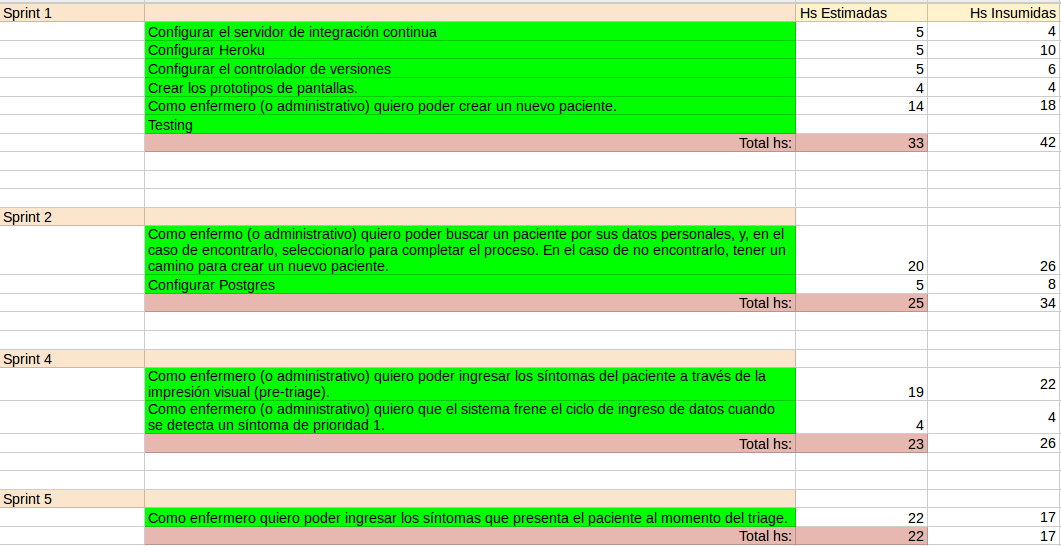
\includegraphics[width=1.2\textwidth]{planificacion.png}}
  \caption{Planificación}
  \label{fig:planificacion}
\end{figure}

A partir de ahí comenzamos con el desarrollo recorriendo las iteraciones planificadas. Al promediar el proyecto hicimos una instalación de prueba en el hospital, y al finalizar el mismo hicimos la instalación definitiva del producto terminado en una máquina de dicha institución.

\subsubsection{Flujo de trabajo en una iteración}
Al inicio de cada iteración estimamos cuanto tiempo nos llevaría cada tarea y enviamos un email con los detalles sobre lo que haríamos durante esa semana. Hacíamos prototipos de las pantallas a realizar que eran validados por el Dr. Reggiani. Dejamos sentado en una hoja de cálculo los detalles de cada tarea: el tiempo de realización estimado, la fecha de realización y el tiempo real insumido (ver figura \ref{fig:tracking}). Luego de cada avance enviamos un reporte por email informando lo realizado y si habían surgido contratiempos. Al finalizar la iteración, enviamos otro email con los detalles de las tareas finalizadas, las que estaban en progreso y las que habían quedado pendientes.

\begin{figure}[h]
  \centerline{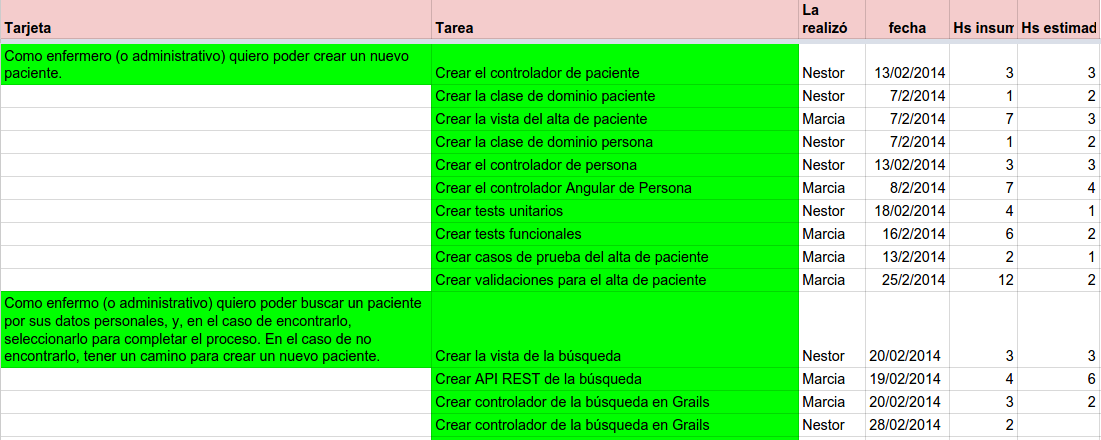
\includegraphics[width=1.2\textwidth]{tracking.png}}
  \caption{\textit{Tracking} de tareas}
  \label{fig:tracking}
\end{figure}

\subsubsection{Herramientas que utilizamos}
Detallamos a continuación las herramientas que utilizamos durante el trabajo.
\begin{itemize}
\item Google Groups\footnote{https://groups.google.com}: comunicación vía email.
\item Google Drive\footnote{https://drive.google.com/}: compartir documentación en línea.
\item Skype\footnote{http://www.skype.com.ar/es/} y Google Hangouts\footnote{https://plus.google.com/hangouts}: comunicación oral de forma remota.
\item Balsamiq\footnote{https://balsamiq.com/}: hacer prototipos de pantallas.
\item Git\footnote{http://git-scm.com/} y Github\footnote{https://github.com/}: versionar y compartir el código (ver sección \ref{cap:repo}).
\item Travis\footnote{https://travis-ci.org/}: servidor de integración continua\footnote{http://es.wikipedia.org/wiki/Integración\_continua}.
\end{itemize}

\subsubsection{Repositorio remoto del código fuente de la aplicación}\label{cap:repo}
El código fuente de la aplicación está disponible en https://github.com/nestor-m/triage

\subsection{Tecnologías}
Todas las tecnologías que utilizamos en el desarrollo de la aplicación son de código abierto. Para desarrollar el \textit{front-end} elegimos AngularJS\footnote{https://angularjs.org/} y para el \textit{back-end} elegimos Grails\footnote{https://grails.org/}.

Cabe aclarar que ambos frameworks cubrieron ampliamente todo lo que nosotros necesitábamos de ellos para hacer este trabajo, por ello sólo utilizamos una pequeña parte de los mismos. Por ejemplo, de Grails casi no utilizamos la parte de las vistas ya que las mismas las desarrollamos del lado del cliente en AngularJS.

Además de estas dos tecnologías utilizamos Bootstrap\footnote{http://getbootstrap.com/} para obtener un diseño amigable para el usuario. Este framework también nos permitió realizar una aplicación \textit{responsive}\footnote{El diseño web adaptable o adaptativo, conocido por las siglas RWD (del inglés, Responsive Web Design) es una filosofía de diseño y desarrollo cuyo objetivo es adaptar la apariencia de las páginas web al dispositivo que se esté utilizando para visualizarla (http://es.wikipedia.org/wiki/Diseño\_web\_adaptable)} que se adapta a cualquier tamaño de pantalla, incluso de teléfonos celulares.

\subsubsection{Sobre la elección de las tecnologías}\label{cap:eleccion_tecnologias}
Como mencionamos anteriormemnte en la sección \ref{cap:itinerario} una de las primeras tareas que realizamos en el proyecto fue la elección de las tecnologías a utilizar. Entre el vasto abanico de posibilidades NodeJS\footnote{http://nodejs.org/} y Grails aparecían como las predilectas ya que son tecnologías modernas y teníamos buenas referencias de ambas. Para decidirnos por una de las dos, desarrollamos un conversor web muy simple de Farenheit a Celcius y en base a los resultados optamos por usar Grails ya que se asemeja más que NodeJS a las tecnologías que veníamos utilizando en las distintas materias a lo largo de la carrera.

Si bien Grails es \textit{full stack}\footnote{Se dice que una tecnología es \textit{full stack} cuando posee todas las herramientas necesarias para desarrollar una aplicación.}, decidimos utilizar una tecnología que resuelva las vistas del lado del cliente, se comunique con el \textit{back-end} mediante una interfaz REST\footnote{La Transferencia de Estado Representacional (Representational State Transfer) o REST es una técnica de arquitectura software para sistemas hipermedia distribuidos como la World Wide Web (http://es.wikipedia.org/wiki/Representational\_State\_Transfer)} 
y sea \textit{responsive}. Así surgió la idea de utilizar AngularJS que cubre ampliamente todos esos requisitos.

Para la elección de la base de datos nos basamos en un tutorial en línea\footnote{https://devcenter.heroku.com/articles/getting-started-with-grails} que recomienda PostgreSQL\footnote{http://www.postgresql.org.es/} como la mejor opción para usar junto a Grails.

\subsubsection{Sobre el \textit{front-end}}
El framework de aplicaciones web AngularJS es desarrollado y mantenido por Google. Es de código abierto y está escrito en JavaScript. La primer versión fue lanzada en el año 2010 y desde ese momento viene ganando espacio en la industria. Este framework es un conjunto de herramientas para la creación de aplicaciones web de una sola página (\textit{single-page applications}). Maneja contenido dinámico y permite extender el vocabulario HTML\footnote{http://es.wikipedia.org/wiki/HTML} obteniendo un entorno más expresivo, legible y práctico para el programador. La filosofía de AngularJS es que la programación declarativa es la que debe utilizarse para generar interfaces de usuario.

\subsubsection{Sobre el \textit{back-end}}
El framework de aplicaciones web Grails es \textit{full stack}, de código abierto y está hecho para la máquina virtual de Java (JVM). Está escrito en Groovy, un lenguaje de programación que a su vez está desarrollado en Java. Uno de sus principios es la convención sobre la configuración que busca decrementar el número de decisiones que un desarrollador necesita tomar, ganando así en simplicidad pero no perdiendo flexibilidad por ello. La primer versión fue lanzada en el año 2006.

Como está desarrollado en Java, Grails es multiplataforma. Además toma de su lenguaje padre tecnologías ampliamente utilizadas en la industria como Hibernate\footnote{http://es.wikipedia.org/wiki/Hibernate}, para la persistencia de datos, y Spring\footnote{http://es.wikipedia.org/wiki/Spring\_Framework}, para la seguridad, la autenticación, las pruebas, la gestión de transacciones, etc.

\subsubsection{Sobre la base de datos}
Para desarrollar una aplicación como la requerida se hizo indispensable utilizar una base de datos para almacenar toda la información ingresada. Los pacientes, los síntomas, las prioridades, los tiempos de espera, etc. son almacenados en una base de datos.

Durante todo el desarrollo de la aplicación utilizamos una base de datos H2\footnote{http://www.h2database.com} que viene embebida en Grails especialmente para utilizar en la etapa de desarrollo. También utilizamos esa tecnología en la instalación de prueba en el hospital. Pero para la instalación definitiva no utilizamos H2 ya que consideramos más apropiado y seguro tener una base de datos independiente del resto del sistema. Por eso utilizamos PostgreSQL\footnote{http://www.postgresql.org.es/} que es un sistema de gestión de bases de datos relacional orientado a objetos.


\subsection{Arquitectura}
Debido a que teníamos que desarrollar una aplicación web capaz de accederse concurrentemente desde varias máquinas al mismo tiempo, decidimos usar una arquitectura cliente-servidor\footnote{http://es.wikipedia.org/wiki/Cliente-servidor} con AngularJS del lado del cliente y Grails del lado del servidor. La comunicación se da mediante peticiones HTTP\footnote{http://es.wikipedia.org/wiki/Hypertext\_Transfer\_Protocol} desde el cliente al servidor y la información viaja en formato JSON\footnote{http://es.wikipedia.org/wiki/JSON}.


\subsubsection{Arquitectura del \textit{front-end}}
El framework AngularJS sigue el patrón de arquitectura Modelo-Vista-Controlador (MVC) de ingeniería de software y alienta la articulación flexible entre la presentación, los datos y los componentes lógicos. Con el uso de la inyección de dependencias, AngularJS lleva servicios tradicionales del lado del servidor, tales como controladores dependientes de la vista, a las aplicaciones web del lado del cliente. En consecuencia, gran parte de la carga en el \textit{backend} se reduce, lo que lleva a aplicaciones web mucho más ligeras.

\subsubsection{Arquitectura del \textit{back-end}}
El framework Grails, al igual que AngularJS, también sigue el patrón de arquitectura MVC. En lo que se refiere a la vista, como en este caso desarrollamos una aplicación de una sola página, entonces tenemos una única pantalla. Por el lado de los controladores tenemos uno por cada clase de dominio. La función principal de los controladores es procesar y responder las peticiones HTTP que llegan desde el lado del cliente. Para hacer esto el controlador se apoya en su clase de dominio (ver figura \ref{fig:diagrama_de_clases}) correspondiente y ésta, a su vez, es la que se encarga de interactuar con la base de datos.

\begin{figure}
\centerline{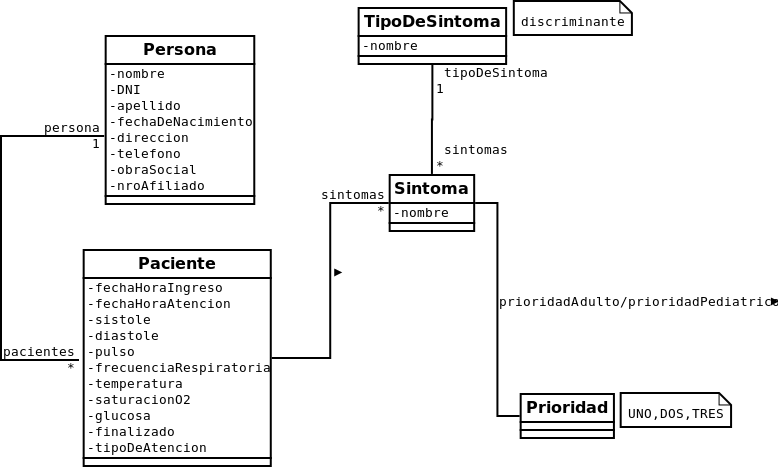
\includegraphics[width=1.2\textwidth]{triage.png}}
\caption{Diagrama de clases del dominio}
\label{fig:diagrama_de_clases}
\end{figure}

\newpage 
\section{Conclusiones}

\paragraph{}
El presente trabajo abordó el planteo, diseño, implementación, desarrollo y puesta en producción de ``Triage, Sistema de gestión para 
sala de Guardia Hospitalaria''

\paragraph{}
La primer conclusión importante que obtuvimos es la facilidad con la que se pudo desarrollar el trabajo gracias a la interacción continua con el cliente y los directores. Este modo de trabajo permitió llevar el enfoque general del desarrollo hacia el producto final que necesita el cliente. 

\paragraph{}
La segunda conclusión que obtuvimos al terminar el desarrollo de este trabajo es que el contenido en general de la carrera nos dió las herramientas y el conocimiento para poder encarar un proyecto de una magnitud mayor a lo aprendido en cualquiera de las materias cursadas. Permitiendo así la familiarización rápida con tecnologías nunca utilizadas.

\paragraph{}
Finalmente queda por mencionar que, como todo diseño, si bien el trabajo efectuado es de calidad y funcionalidad, queda abierto a mejoras y agregación de nuevas funcionalidades en futuros TIPs.





\newpage 

\begin{thebibliography}{3} 
\bibitem{Derlet} Derlet R, Kinser D, Lou R, et al. Prospective identification and triage of nonemergency patients out of an Emergency Department: a 5 years study. Ann Emerg Med 1996; 25:215-223.
\bibitem{Manual} Manual de procedimiento. Recepción,  Acogida y Clasificación.  MSPBS. Paraguay 2011.
\bibitem{Shore} Shore J, Warden S, The Art of Agile Development, O’Reilly Media, 2007.

\end{thebibliography}
 


\end{document}
